\documentclass{article}
\usepackage[utf8]{inputenc}

\usepackage{caption}
\usepackage{graphicx, subfig}
\usepackage{subfigure}
\usepackage{amsmath}
\usepackage{mathrsfs}
\usepackage{amsfonts}
\usepackage{natbib}
\usepackage{graphicx}
\usepackage{amssymb}
\usepackage{upgreek}
\usepackage{listings}
\usepackage{xcolor}
\usepackage{dsfont}


\title{Homework #3}
\author{Coffee Automaton}
\date{September 2019}

\begin{document}

\maketitle

\textbf{Exercise 1}
It's trivial that $T$ is a subgraph of $G$, and $T_{c}$ is a subgraph of $G_{c}$.

So for two vertices $u,v$, if $u,v$ are connected in $T_{c}$, they are must connected in $G_{c}$, because $T_{c}$ is a subgraph of $G_{c}$.

If $u,v$ are not connected in $T_{c}$, they are not connected in $G_{c}$. A simple proof: because $T$ is a minimum spanning tree of $G$, so all vertices are connected in $T$. If $u,v$ are not connected in $T_{c}$, there is at least an edge that connect $u$ and $v$ which weights bigger than $c$. Assume $u,v$ are connected in $G_{c}$, then there is an path to connect $u$ and $v$ that every edge's weight is less or equal to $c$. So we can find a tree that is a spanning tree of $G$, which has smaller weight than $T$. But $T$ is the MST, so it is a contradiction.

So $T_c$ and $G_c$ have exactly the same connected components. 


~\\
\textbf{Exercise 2}
Considering the Kruskal's algorithm, all MSTs have $n-1$ edges, and have same amount of edges with weight 1, weight 2, .... , weight c. So all $T_c$ have same amount of edges, that $m_{c}(T) = m_{c}(T')$.

~\\
\textbf{Exercise 3}
Considering the Kruskal's algorithm, each time we chooose edge of fixed weight and cycle $n-1$ times. Because no two of edges have same weight, what we choose is determinate and unique. So there is exactly one MST.

~\\
\textbf{Exercise 4}
The multigraph is showed in figure \ref{img} with labeled.

Because we want a spanning tree, so edge $a$ is a must, and choose two edges of $b,c,d$, three edges of $e,f,g,h$. And we have three choices in $d$, two choices in $e$, so we have 
$(2*3 + 1)*(3*2 + 1) = 49$ spanning trees.


\begin{figure}
		\centering
		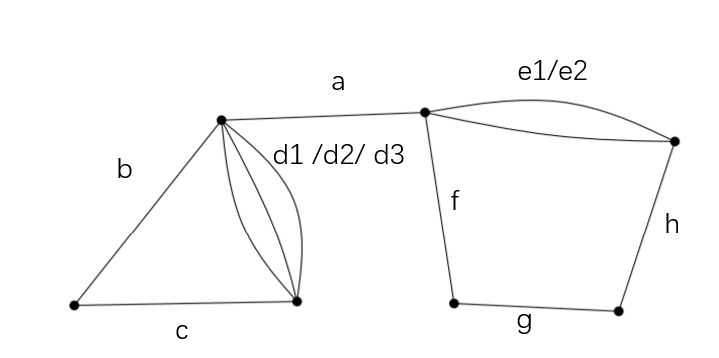
\includegraphics[width=0.5\textwidth]{3.png}
		\caption{
		multigraph in Exercise 4} 
		\label{img}
	\end{figure}

~\\
\textbf{Exercise 5}


\end{document}
